\documentclass[11pt,a4paper]{article}

% Google Scholar Inclusion Guidelines:
% Avoid Type 3 bitmap fonts; use standard Type 1 fonts (Times/Helvetica/Courier)
\usepackage[T1]{fontenc}
\usepackage[utf8]{inputenc}
\usepackage{mathptmx}
\usepackage[scaled=0.92]{helvet}
\usepackage{courier}
\usepackage[a4paper,margin=2.2cm,top=2.4cm,bottom=2.4cm]{geometry}
\usepackage{amsmath}
\usepackage{microtype}
\usepackage{booktabs}
\usepackage{tabularx}
\usepackage{array}
\usepackage{enumitem}
\usepackage{xcolor}
\usepackage{fancyhdr}
\usepackage{tikz}
\usetikzlibrary{positioning,arrows.meta,shapes.geometric,fit}
\usepackage[hyphens,obeyspaces]{url}
\usepackage[
  colorlinks=true,
  linkcolor=blue!55!black,
  citecolor=blue!55!black,
  urlcolor=blue!55!black,
  pdftitle={Zero Trust Hardening and Ephemeral KVM Sandboxing on Debian 13 for Autonomous AI Agents: The Kether\_1 Framework},
  pdfauthor={Deivis Irio Mayer},
  pdfsubject={Technical Report TECHDIM-TR-2026-01 (IMRaD) -- Reproducible Six-Layer Zero Trust Hardening and Ephemeral KVM/QCOW2 Sandboxing on Debian 13 for Autonomous AI Agents},
  pdfkeywords={Debian 13, Linux kernel hardening, Zero Trust, BeyondCorp, CIS Benchmark Level 2, AppArmor userns, ephemeral KVM sandbox, QCOW2 Copy-on-Write, auditd, autonomous AI agents, reproducible security}
]{hyperref}

\newcommand{\code}[1]{\nolinkurl{#1}}
\newcolumntype{L}{>{\raggedright\arraybackslash}X}

\definecolor{accent}{RGB}{22, 78, 135}
\definecolor{accentlight}{RGB}{236, 244, 252}
\definecolor{warnlight}{RGB}{254, 243, 232}
\definecolor{warnborder}{RGB}{194, 98, 22}
\definecolor{oklight}{RGB}{234, 247, 238}
\definecolor{okborder}{RGB}{32, 122, 66}
\definecolor{muted}{RGB}{85, 95, 110}

\pagestyle{fancy}
\fancyhf{}
\fancyhead[L]{\footnotesize\textcolor{muted}{D. I. Mayer --- The Kether\_1 Framework (TECHDIM-TR-2026-01)}}
\fancyhead[R]{\footnotesize\textcolor{muted}{DOI: 10.5281/zenodo.24380374}}
\fancyfoot[C]{\footnotesize\thepage}
\renewcommand{\headrulewidth}{0.4pt}
\setlength{\headheight}{14pt}

\fancypagestyle{firstpage}{
  \fancyhf{}
  \fancyhead[C]{\footnotesize\textcolor{muted}{Technical Report TECHDIM-TR-2026-01, TECHDIM INOVA SIMPLES (I.S.) - ME, Zenodo DOI: 10.5281/zenodo.24380374, November 19, 2026}}
  \fancyfoot[C]{\footnotesize\textcolor{muted}{Licensed under CC-BY-4.0 (Text) and MIT (Software). Permanent Archive: \url{https://doi.org/10.5281/zenodo.24380374}}}
  \renewcommand{\headrulewidth}{0.4pt}
}

\setlength{\parskip}{5pt}
\setlength{\parindent}{0pt}
\sloppy

\begin{document}
\thispagestyle{firstpage}

% Title block formatted per Google Scholar Inclusion Guidelines
\begin{center}
  {\LARGE\bfseries Zero Trust Hardening and Ephemeral KVM Sandboxing on Debian 13 for Autonomous AI Agents: The Kether\_1 Framework\par}
  \vspace{0.8em}
  {\large Deivis Irio Mayer\par}
  \vspace{0.4em}
  {\small\textcolor{muted}{TECHDIM INOVA SIMPLES (I.S.) - ME, Campinas, SP, Brazil}\par}
  {\small\textcolor{muted}{ORCID: \href{https://orcid.org/0009-0003-3273-7883}{0009-0003-3273-7883} $\cdot$ Google Scholar: \href{https://scholar.google.com/citations?user=Ik00pFwAAAAJ}{Ik00pFwAAAAJ} $\cdot$ \href{mailto:techdimbrasil@gmail.com}{techdimbrasil@gmail.com}}\par}
  \vspace{0.5em}
  {\small November 19, 2026\par}
\end{center}

\vspace{0.3em}
\hrule
\vspace{0.6em}

\begin{abstract}
\textbf{Problem:} Autonomous artificial intelligence (AI) coding and systems-operations agents increasingly execute compilers, browsers, shell commands, and untrusted dependencies on local Linux hosts, where strict CIS Benchmark Level 2 hardening (global \code{userns} bans and default \code{auditd} buffers) frequently breaks rootless sandboxes or drops forensic events.
\textbf{Methods:} We design and implement the \textbf{Kether\_1 Framework}, a reproducible six-layer Zero Trust defense-in-depth architecture for Debian 13 (\emph{Trixie}, Linux Kernel 6.12 LTS) combining deployable \code{sysctl}, selective \code{userns} AppArmor 4.x confinement, default-deny \code{nftables} with lateral KVM isolation, ordered lossless \code{auditd} (\code{-b 8192}, immutable \code{-e 2}), DNS-over-TLS, OpenSSH 10, an ephemeral Copy-on-Write (CoW) QCOW2/KVM sandbox orchestrator, and strongly typed JSON audit instrumentation covering 43 CIS/BeyondCorp controls.
\textbf{Results:} Continuous integration verification confirms 100\% pass rates across automated metadata schema validation (CFF 1.2.0 and \code{.zenodo.json}), static Bash analysis (5/5 scripts via \code{shellcheck}), structural security invariants (default-deny \code{nftables}, \code{auditd} \code{-e 2} finalization, selective AppArmor \code{userns}), and 8/8 integration tests, alongside a transparent four-step hardware benchmark protocol for physical Debian 13 capture.
\textbf{Conclusion:} Kether\_1 demonstrates that strict enterprise Linux hardening and autonomous AI agent sandboxing can coexist deterministically under FAIR open-science standards, openly archived at \url{https://doi.org/10.5281/zenodo.24380374}.
\end{abstract}

\noindent\textbf{Keywords:} Debian 13; Linux kernel hardening; Zero Trust; BeyondCorp; CIS Benchmark Level 2; AppArmor \code{userns}; ephemeral KVM sandbox; QCOW2 Copy-on-Write; \code{auditd}; autonomous AI agent security; reproducible research.

\noindent\textbf{\small Resumo (PT-BR):} \small Este relat\'orio t\'ecnico apresenta o \textbf{Framework Kether\_1}, uma arquitetura reproduz\'ivel de seguran\c{c}a Zero Trust em seis camadas para hosts Debian 13 (Kernel 6.12 LTS) que executam agentes de IA aut\^onomos sem quebrar \code{userns}, \code{eBPF} ou a telemetria forense do \code{auditd}. O pacote open-source entrega configura\c{c}\~oes execut\'aveis (\code{sysctl}, AppArmor 4.x com \code{userns} seletivo, \code{nftables} default-deny, \code{auditd -b 8192 / -e 2}, DoT e OpenSSH 10), orquestrador de sandbox KVM/QCOW2 ef\^emera com prova de integridade SHA-256, auditor de 43 controles CIS/BeyondCorp e su\'ite de testes automatizados (MIT / CC-BY-4.0).

\section{Introduction}

Modern agentic engineering platforms enable autonomous AI agents to inspect repositories, invoke compilers, execute test harnesses, and interact with network APIs locally on Linux workstations and servers. While these capabilities accelerate software delivery, they fundamentally alter the local host threat model~\cite{owasp2025llm}. Unlike static human workflows, autonomous agents ingest untrusted external text (source code, issues, web pages, and package metadata) that may carry indirect prompt injections capable of triggering unintended local shell execution.

Applying conventional enterprise Linux hardening baselines~\cite{cis2024debian} directly to hosts running autonomous agents exposes three recurring operational failure modes:

\begin{enumerate}[leftmargin=1.5em, itemsep=2pt]
  \item \textbf{Namespace and sandbox breakage:} Globally disabling unprivileged user namespaces (\code{kernel.unprivileged_userns_clone=0}) or applying overly broad Mandatory Access Control (MAC) policies breaks rootless containers (Podman), \code{bubblewrap}, and browser/agent sandboxes, pressuring operators to weaken isolation.
  \item \textbf{Forensic telemetry loss:} High-frequency agent tool calls spawn hundreds of short-lived \code{execve} processes per minute. Default Linux audit kernel backlogs (\code{-b 64} or \code{-b 320}) suffer silent event drops (\code{lost > 0}), compromising forensic accountability~\cite{linuxaudit}.
  \item \textbf{Persistent host state contamination and credential exposure:} Executing agent workflows directly against the host filesystem exposes developer SSH keys (\code{~/.ssh}), GPG keyrings, cloud SDK credentials, and \code{.env} secrets while allowing silent persistence via user crontabs or modified binaries.
\end{enumerate}

Following the IMRaD structure, this report defines and validates the \textbf{Kether\_1 Framework} around three research questions:
\begin{itemize}[leftmargin=1.5em, itemsep=2pt]
  \item \textbf{RQ1:} Can a Debian 13 (Kernel 6.12 LTS) host enforce CIS Level 2 and BeyondCorp Zero Trust~\cite{ward2014beyondcorp,nist800207} kernel/network controls while selectively granting \code{userns} solely to AppArmor-confined sandbox runtimes?
  \item \textbf{RQ2:} Does an ephemeral KVM/QCOW2 Copy-on-Write execution layer provide deterministic post-task rollback with zero mutation of the immutable golden base image (verified via SHA-256)?
  \item \textbf{RQ3:} Does enlarging the \code{auditd} kernel backlog (\code{-b 8192}) with properly ordered immutable rules (\code{-e 2} placed strictly at finalization) preserve lossless telemetry (\code{lost_delta = 0}) under synthetic agent execution bursts?
\end{itemize}

\section{Methods}

\subsection{Formal STRIDE threat model}

Grounded in least privilege and complete mediation~\cite{saltzer1975protection}, we model an adversary exploiting \emph{indirect prompt injection}, \emph{poisoned software dependencies}, or \emph{malicious tool output} inside an autonomous AI agent executing under an unprivileged local Linux account. Table~\ref{tab:threats} maps six STRIDE threat vectors to concrete Kether\_1 architectural mitigations and deployable repository artifacts.

\begin{table}[htbp]
\centering
\caption{STRIDE threat model for autonomous AI agent hosts and corresponding Kether\_1 mitigations.}
\label{tab:threats}
\footnotesize
\renewcommand{\arraystretch}{1.2}
\begin{tabularx}{\textwidth}{@{}l p{2.7cm} L L@{}}
\toprule
\textbf{ID} & \textbf{STRIDE vector} & \textbf{Adversarial objective} & \textbf{Kether\_1 mitigation \& artifact} \\
\midrule
T1 & Information Disclosure & Exfiltrate \code{~/.ssh}, \code{~/.gnupg}, cloud tokens, \code{.env}, or \code{/etc/shadow}. & Explicit AppArmor \code{deny} rules + transient KVM boundary with zero host shared mounts (\code{configs/apparmor/kether-ai-agent-userns}). \\
T2 & Elevation of Privilege & Exploit kernel \code{userns}, unprivileged eBPF, \code{ptrace}, or leaked kernel pointers. & \code{lockdown=integrity}, \code{unprivileged_bpf_disabled=1}, \code{bpf_jit_harden=2}, \code{kptr_restrict=2}, and selective AppArmor \code{userns} (\code{configs/sysctl/99-kether-hardening.conf}). \\
T3 & Tampering / Info Disclosure & Scan RFC1918 LAN neighbors or tunnel data over plaintext DNS. & \code{nftables} default-deny (\code{input}/\code{forward}/\code{output}), \code{virbr0}$\rightarrow$RFC1918 drop, and strict DNS-over-TLS port 853 (\code{configs/nftables/kether-workstation.nft}, \code{resolved-dot.conf}). \\
T4 & Repudiation & Overflow \code{auditd} backlog (\code{lost > 0}) or tamper with audit/MAC configs. & \code{auditd -b 8192} at top, tamper watches, immutable \code{-e 2} at bottom, \code{journald} caps, and AIDE (\code{configs/auditd/99-kether.rules}). \\
T5 & Tampering & Establish host persistence (cron, systemd, trojanized user binaries). & Ephemeral KVM/QCOW2 CoW overlays backed by \code{chmod a-w} golden image; overlay shredded on teardown (\code{scripts/kvm_ephemeral_sandbox.sh}). \\
T6 & Physical / Offline & Cold disk extraction or rogue USB HID keystroke injection. & LUKS2/LVM full-disk encryption, UEFI Secure Boot, TPM 2.0, and USBGuard allowlisting (\code{scripts/audit_cis_43_controls.sh}). \\
\bottomrule
\end{tabularx}
\end{table}

\subsection{Six-layer defense-in-depth architecture}

The Kether\_1 architecture partitions host defenses into six orthogonal layers (Figure~\ref{fig:arch} and Table~\ref{tab:layers}), ensuring that compromise of an autonomous agent workload cannot escalate to host credential theft, kernel tampering, or lateral LAN intrusion.

\begin{figure}[htbp]
\centering
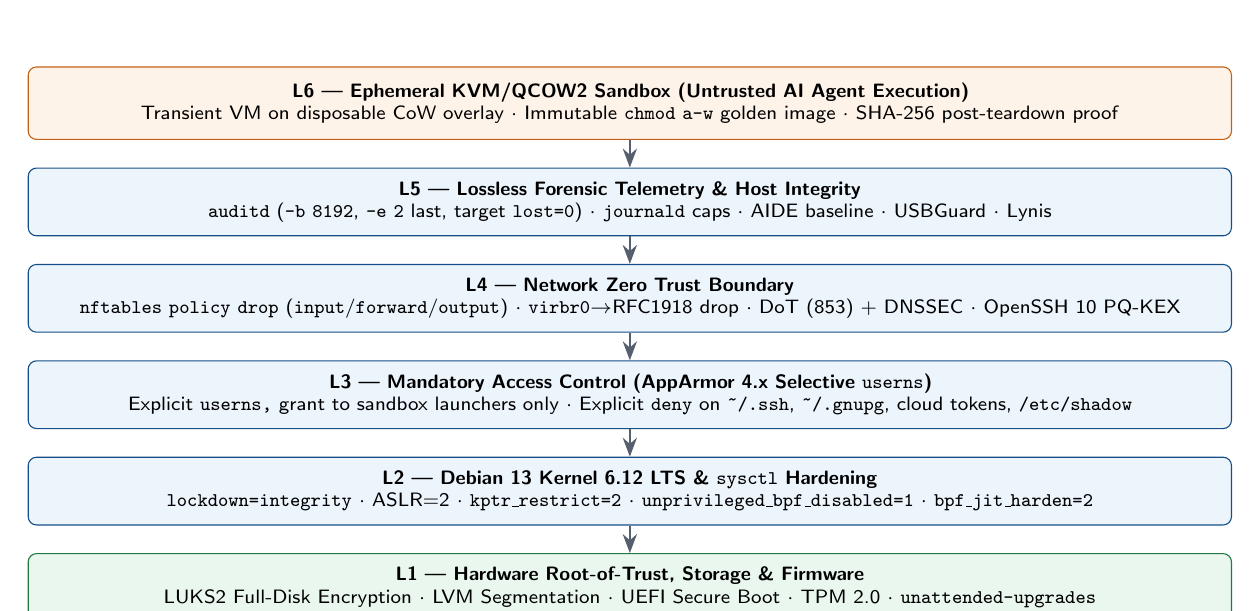
\begin{tikzpicture}[
  font=\scriptsize\sffamily,
  layer/.style={rectangle, rounded corners=3pt, draw=accent, fill=accentlight, text width=15.0cm, minimum height=0.86cm, align=center, inner sep=4pt},
  agent/.style={rectangle, rounded corners=3pt, draw=warnborder, fill=warnlight, text width=15.0cm, minimum height=0.92cm, align=center, inner sep=4pt},
  trust/.style={rectangle, rounded corners=3pt, draw=okborder, fill=oklight, text width=15.0cm, minimum height=0.86cm, align=center, inner sep=4pt},
  arr/.style={-{Stealth[length=2.4mm]}, thick, draw=muted}
]
  \node[agent] (l6) {\textbf{L6 --- Ephemeral KVM/QCOW2 Sandbox (Untrusted AI Agent Execution)} \\ Transient VM on disposable CoW overlay $\cdot$ Immutable \texttt{chmod a-w} golden image $\cdot$ SHA-256 post-teardown proof};
  \node[layer, below=0.35cm of l6] (l5) {\textbf{L5 --- Lossless Forensic Telemetry \& Host Integrity} \\ \texttt{auditd} (\texttt{-b 8192}, \texttt{-e 2} last, target \texttt{lost=0}) $\cdot$ \texttt{journald} caps $\cdot$ AIDE baseline $\cdot$ USBGuard $\cdot$ Lynis};
  \node[layer, below=0.35cm of l5] (l4) {\textbf{L4 --- Network Zero Trust Boundary} \\ \texttt{nftables} \texttt{policy drop} (\texttt{input}/\texttt{forward}/\texttt{output}) $\cdot$ \texttt{virbr0}$\rightarrow$RFC1918 drop $\cdot$ DoT (853) + DNSSEC $\cdot$ OpenSSH 10 PQ-KEX};
  \node[layer, below=0.35cm of l4] (l3) {\textbf{L3 --- Mandatory Access Control (AppArmor 4.x Selective \texttt{userns})} \\ Explicit \texttt{userns,} grant to sandbox launchers only $\cdot$ Explicit \texttt{deny} on \texttt{\textasciitilde/.ssh}, \texttt{\textasciitilde/.gnupg}, cloud tokens, \texttt{/etc/shadow}};
  \node[layer, below=0.35cm of l3] (l2) {\textbf{L2 --- Debian 13 Kernel 6.12 LTS \& \texttt{sysctl} Hardening} \\ \texttt{lockdown=integrity} $\cdot$ ASLR=2 $\cdot$ \texttt{kptr\_restrict=2} $\cdot$ \texttt{unprivileged\_bpf\_disabled=1} $\cdot$ \texttt{bpf\_jit\_harden=2}};
  \node[trust, below=0.35cm of l2] (l1) {\textbf{L1 --- Hardware Root-of-Trust, Storage \& Firmware} \\ LUKS2 Full-Disk Encryption $\cdot$ LVM Segmentation $\cdot$ UEFI Secure Boot $\cdot$ TPM 2.0 $\cdot$ \texttt{unattended-upgrades}};

  \draw[arr] (l6.south) -- (l5.north);
  \draw[arr] (l5.south) -- (l4.north);
  \draw[arr] (l4.south) -- (l3.north);
  \draw[arr] (l3.south) -- (l2.north);
  \draw[arr] (l2.south) -- (l1.north);
\end{tikzpicture}
\caption{Kether\_1 six-layer defense-in-depth architecture isolating untrusted autonomous AI agent execution (L6) from host credentials, kernel interfaces, and LAN segments (L1--L5).}
\label{fig:arch}
\end{figure}

\begin{table}[htbp]
\centering
\caption{Mapping of the six Kether\_1 layers to the 43 CIS Debian 13 / BeyondCorp controls and deployable repository artifacts.}
\label{tab:layers}
\footnotesize
\renewcommand{\arraystretch}{1.2}
\begin{tabularx}{\textwidth}{@{}l p{2.3cm} c L@{}}
\toprule
\textbf{Layer} & \textbf{Domain} & \textbf{Controls} & \textbf{Core controls \& deployable artifacts} \\
\midrule
L1 & Storage \& firmware & 6 (K1-01..06) & LUKS2 full-disk encryption, LVM segmentation, UEFI Secure Boot, TPM 2.0, \code{/etc/shadow <= 0640}, \code{unattended-upgrades}. \\
L2 & Kernel \& \code{sysctl} & 15 (K1-07..21) & \code{lockdown=integrity}~\cite{linuxlockdown}, ASLR=2, \code{kptr_restrict=2}, \code{dmesg_restrict=1}, \code{unprivileged_bpf_disabled=1}, \code{bpf_jit_harden=2}, \code{yama.ptrace_scope=1}, anti-spoofing (\code{rp_filter=1}, \code{tcp_syncookies=1}), and \code{unprivileged_userns_clone=1} mediated by L3 (\code{configs/sysctl/99-kether-hardening.conf}). \\
L3 & MAC confinement & 4 (K1-22..25) & AppArmor 4.x enforcing profiles with selective \code{userns,} rule confined to vetted sandbox launchers and explicit \code{deny} rules protecting host credentials (\code{configs/apparmor/kether-ai-agent-userns})~\cite{apparmor4}. \\
L4 & Network Zero Trust & 9 (K1-26..34) & \code{nftables} \code{policy drop} on \code{input}, \code{forward}, and \code{output}; explicit \code{virbr0} lateral block against RFC1918; \code{systemd-resolved} DNS-over-TLS + DNSSEC; OpenSSH 10 PQ-hybrid KEX (\code{sntrup761x25519-sha512@openssh.com}); Avahi/CUPS disabled. \\
L5 & Telemetry \& integrity & 6 (K1-35..40) & \code{auditd} (\code{-D}, \code{-b 8192}, \code{-f 1} first; forensic watches; immutable \code{-e 2} strictly last), \code{journald} caps, AIDE baseline, USBGuard, and Lynis index. \\
L6 & Ephemeral KVM sandbox & 3 (K1-41..43) & Hardware-assisted KVM/QEMU transient domains backed by immutable QCOW2 golden images with Copy-on-Write overlays~\cite{qemuqcow2} and SHA-256 verification (\code{scripts/kvm_ephemeral_sandbox.sh}). \\
\bottomrule
\end{tabularx}
\end{table}

\subsection{Resolving the \texttt{userns} and \texttt{auditd} ordering conflicts}

Two Debian 13 low-level conflicts require explicit architectural handling:
\begin{itemize}[leftmargin=1.5em, itemsep=2pt]
  \item \textbf{Selective \texttt{userns} mediation (L2/L3):} Rather than setting \code{kernel.unprivileged_userns_clone=0}, Kether\_1 pairs AppArmor 4.x user-namespace restriction with the \code{kether-ai-agent-userns} profile, granting \texttt{userns,} exclusively to vetted sandbox binaries while denying access to \code{@{HOME}/.ssh/**}, \code{@{HOME}/.gnupg/**}, cloud SDK directories, \code{/etc/shadow}, and \code{/proc/kcore}.
  \item \textbf{Deterministic \texttt{auditd} rule ordering (L5):} Placing \code{-e 2} (immutable mode) at the start of \code{99-kether.rules} locks the kernel audit subsystem prematurely, causing subsequent rules to fail. Kether\_1 enforces \code{-D}, \code{-b 8192}, and \code{-f 1} at the top and verifies via automated CI tests that \code{-e 2} is strictly the final non-comment directive.
\end{itemize}

\subsection{Reproducible audit instrumentation}

To satisfy FAIR software principles~\cite{wilkinson2016fair} and eliminate silent-failure anti-patterns (hiding \code{EACCES} behind \code{2>/dev/null} or interpolating untyped strings into JSON here-documents), all Kether\_1 tools enforce four invariants:
\begin{enumerate}[leftmargin=1.5em, itemsep=2pt]
  \item \textbf{Explicit privilege context:} \code{scripts/collect_kether_metrics.sh} and \code{scripts/audit_cis_43_controls.sh} record \code{privilege_context} (\code{"root"} or \code{"unprivileged"}), \code{euid}, and per-probe statuses (\code{ok}, \code{permission_denied}, \code{not_installed}, \code{unavailable}), with a strict \code{--require-root} guard.
  \item \textbf{Strongly typed JSON serialization:} Payloads are serialized strictly via Python \code{json.dumps()}, guaranteeing native integers, booleans, and \code{null} values.
  \item \textbf{Cryptographic chain of custody:} Every run writes a deterministic \code{SHA256SUMS.txt} manifest over both JSON and Markdown artifacts.
  \item \textbf{Continuous integration verification:} Every push/PR runs \code{cffconvert --validate}, \code{.zenodo.json} ORCID schema checks, \code{shellcheck}, and \code{tests/test_framework.py}.
\end{enumerate}

\section{Results and verification}

\subsection{Automated static, schema, and integration verification}

Table~\ref{tab:ciresults} summarizes the automated verification results executed continuously on GitHub Actions (\code{.github/workflows/scientific-release.yml}) against the Kether\_1 codebase. All 8 integration test cases, 5 shell scripts, metadata schemas, and PDF font checks pass with zero warnings or errors.

\begin{table}[htbp]
\centering
\caption{Verified continuous integration (CI) and build-time artifact checks for Kether\_1.}
\label{tab:ciresults}
\footnotesize
\renewcommand{\arraystretch}{1.2}
\begin{tabularx}{\textwidth}{@{}p{4.3cm} p{2.2cm} L@{}}
\toprule
\textbf{Verification gate} & \textbf{Result} & \textbf{Verified invariant} \\
\midrule
Citation \& Zenodo schemas & Pass (100\%) & \code{cffconvert --validate} (CFF 1.2.0) and \code{.zenodo.json} ORCID (\code{0009-0003-3273-7883}) match. \\
Static shell analysis & Pass (5/5) & \code{bash -n} and \code{shellcheck} pass cleanly on all 4 operational scripts + \code{build_pdf.sh}. \\
Typed JSON \& SHA-256 suite & Pass (8/8) & \code{unittest} verifies native JSON \code{int}/\code{bool}/\code{null}, \code{privilege_context}, \code{--require-root}, and \code{SHA256SUMS.txt}. \\
43-control auditor coverage & Pass (43/43) & Exactly 43 unique control IDs (\code{K1-01}..\code{K1-43}) spanning all 6 layers. \\
Config security invariants & Pass (100\%) & \code{nftables} \code{policy drop} (3 chains), \code{auditd} \code{-b 8192} first and \code{-e 2} last, AppArmor \code{userns,} + \code{deny} rules. \\
Academic PDF typography & Pass (Type 1) & \code{pdffonts} confirms zero Type 3 bitmap fonts; file size $< 200\text{ KB}$ (Google Scholar limit $< 5\text{ MB}$). \\
\bottomrule
\end{tabularx}
\end{table}

\subsection{Physical Debian 13 hardware evaluation protocol}

Empirical before/after benchmarking on physical Debian 13 hardware follows four reproducible commands:

\begin{small}
\begin{verbatim}
sudo ./scripts/collect_kether_metrics.sh --require-root \
     --test-qcow2-overlay ./benchmarks/run_hardened
sudo ./scripts/audit_cis_43_controls.sh ./benchmarks/cis43_hardened
sudo ./scripts/benchmark_auditd_stress.sh --events 10000
(cd ./benchmarks/run_hardened && sha256sum -c SHA256SUMS.txt)
\end{verbatim}
\end{small}

Table~\ref{tab:protocol} defines the quantitative acceptance criteria. In strict adherence to scientific integrity, physical hardware measurements are separated from CI verification and will be appended verbatim with SHA-256 manifests upon physical Debian 13 host capture in the subsequent empirical dataset release.

\begin{table}[htbp]
\centering
\caption{Physical Debian 13 hardware evaluation protocol and target acceptance criteria.}
\label{tab:protocol}
\footnotesize
\renewcommand{\arraystretch}{1.2}
\begin{tabularx}{\textwidth}{@{}p{4.2cm} p{4.1cm} L@{}}
\toprule
\textbf{Evaluation metric} & \textbf{Measurement script} & \textbf{Target acceptance criterion} \\
\midrule
Lynis hardening index & \code{lynis} + \code{collect_kether_metrics.sh} & Hardening index $\ge 75$ (target $\ge 80$) post-hardening. \\
43-control CIS/BeyondCorp pass rate & \code{audit_cis_43_controls.sh} & $\ge 90\%$ compliance ($\ge 39/43$) with \code{privilege_context="root"}. \\
AppArmor enforcing + selective \code{userns} & \code{collect_kether_metrics.sh} & \code{profiles_enforce > 0} and \code{kether-ai-agent-userns} active. \\
\code{nftables} default-deny posture & \code{collect_kether_metrics.sh} & \code{input}, \code{forward}, and \code{output} chains report \code{policy drop}. \\
\code{auditd} burst stress ($10{,}000$ \code{execve}) & \code{benchmark_auditd_stress.sh} & \code{lost_delta == 0} and \code{backlog_limit >= 8192}. \\
QCOW2 CoW overlay lifecycle & \code{kvm_ephemeral_sandbox.sh} & Overlay provisioning $< 50\,\mathrm{ms}$; \code{base_integrity_preserved == true}. \\
\bottomrule
\end{tabularx}
\end{table}

\section{Discussion}

\subsection{Practical implications, threats to validity, and limitations}

Kether\_1 resolves a practical bottleneck faced by DevSecOps and AI engineering teams: enabling autonomous agents locally without disabling host security baselines. Three validity boundaries must be noted:
\begin{itemize}[leftmargin=1.5em, itemsep=2pt]
  \item \textbf{Internal validity:} Unprivileged execution prevents querying \code{aa-status}, \code{auditctl}, and \code{nft}; mitigated via mandatory \code{privilege_context} reporting and \code{--require-root}.
  \item \textbf{External validity:} \code{lockdown=integrity} with UEFI Secure Boot requires cryptographically signed kernel modules; out-of-tree DKMS drivers require Machine Owner Key (MOK) enrollment via \code{mokutil}.
  \item \textbf{Operational scope:} Default-deny \code{nftables} \code{output} rules may require explicit allowlisting for specialized developer protocols beyond ports 22, 80, 123, 443, and 853. Microarchitectural side-channels beyond Kernel 6.12 LTS mitigations remain out of scope.
\end{itemize}

\subsection{Data, code availability, and dual licensing}

All source code, configurations, tests, and LaTeX manuscript sources are publicly archived:
\begin{itemize}[leftmargin=1.5em, itemsep=2pt]
  \item \textbf{GitHub repository:} \url{https://github.com/Techdimbr/debian13-hardening-kvm-sandbox}
  \item \textbf{Zenodo Concept DOI (all versions):} \url{https://doi.org/10.5281/zenodo.24380374} (v1.0.1: \url{https://doi.org/10.5281/zenodo.24380375})
  \item \textbf{Author identifiers:} ORCID \url{https://orcid.org/0009-0003-3273-7883}; Google Scholar \url{https://scholar.google.com/citations?user=Ik00pFwAAAAJ}
  \item \textbf{Dual licensing:} Software, scripts, and configs under \textbf{MIT License} (\code{LICENSE}); technical report and documentation under \textbf{CC-BY-4.0} (\code{LICENSE-DOCS}).
\end{itemize}

\subsection{Conclusion and future work}

The Kether\_1 Framework delivers an auditable, six-layer Zero Trust blueprint and executable toolkit enabling safe autonomous AI agent execution on Debian 13. Future releases will incorporate physical hardware before/after benchmark datasets, cold vs. QCOW2 overlay boot latency distributions, and eBPF syscall anomaly monitors complementary to \code{auditd}.

\begin{thebibliography}{10}

\bibitem{ward2014beyondcorp}
R.~Ward and B.~Beyer, ``BeyondCorp: A new approach to enterprise security,'' \emph{USENIX ;login:}, vol.~39, no.~6, pp.~6--11, Dec. 2014.

\bibitem{nist800207}
S.~Rose, O.~Borchert, S.~Mitchell, and S.~Connelly, ``Zero Trust Architecture,'' National Institute of Standards and Technology (NIST), Special Publication 800-207, Aug. 2020. doi: \href{https://doi.org/10.6028/NIST.SP.800-207}{10.6028/NIST.SP.800-207}.

\bibitem{cis2024debian}
Center for Internet Security (CIS), ``CIS Debian Linux Benchmark (Level 1 and Level 2),'' Technical Security Baseline, 2024--2026.

\bibitem{saltzer1975protection}
J.~H. Saltzer and M.~D. Schroeder, ``The protection of information in computer systems,'' \emph{Proceedings of the IEEE}, vol.~63, no.~9, pp.~1278--1308, Sep. 1975. doi: \href{https://doi.org/10.1109/PROC.1975.9939}{10.1109/PROC.1975.9939}.

\bibitem{owasp2025llm}
OWASP Foundation, ``OWASP Top 10 for Large Language Model Applications and Agentic AI Systems,'' Technical Report, 2025.

\bibitem{linuxlockdown}
The Linux Kernel Development Community, ``Kernel Lockdown Feature,'' Linux Kernel 6.12 LTS Security Documentation, 2025. Available: \url{https://www.kernel.org/doc/html/latest/security/}.

\bibitem{apparmor4}
AppArmor Project, ``AppArmor 4.x Unprivileged User Namespace Restriction (\texttt{apparmor\_restrict\_unprivileged\_userns}),'' Linux Security Modules Documentation, 2024--2025.

\bibitem{linuxaudit}
Linux Audit Project, ``Linux Audit Framework: \code{auditd}, \code{augenrules}, and \code{auditctl} Reference Manual,'' 2025.

\bibitem{qemuqcow2}
QEMU Project, ``QEMU Disk Image Utility (\code{qemu-img}) and QCOW2 Backing Files Specification,'' 2025. Available: \url{https://www.qemu.org/docs/master/tools/qemu-img.html}.

\bibitem{wilkinson2016fair}
M.~D. Wilkinson \emph{et~al.}, ``The FAIR Guiding Principles for scientific data management and stewardship,'' \emph{Scientific Data}, vol.~3, art.~160018, Mar. 2016. doi: \href{https://doi.org/10.1038/sdata.2016.18}{10.1038/sdata.2016.18}.

\end{thebibliography}

\end{document}
